\documentclass[aspectratio=169]{beamer}

\usetheme{Madrid}
\usecolortheme{default}

\usepackage[T1]{fontenc}
\usepackage{lmodern}
\usepackage{graphicx}
\usepackage{svg}
\usepackage{booktabs}
\usepackage{tikz}
\usetikzlibrary{arrows.meta, positioning, calc}

\graphicspath{{assets/images/}}
\svgpath{{assets/svg/}}
\svgsetup{
  inkscapelatex=false,
  inkscapepath=build/svg-inkscape/
}

\definecolor{tokenblue}{HTML}{DCEBFA}
\definecolor{tokenblueborder}{HTML}{2B5797}
\definecolor{tokenorange}{HTML}{FCE8D5}
\definecolor{tokenorangeborder}{HTML}{B85C00}
\definecolor{tokengreen}{HTML}{E4F3E5}
\definecolor{tokengreenborder}{HTML}{2E7D32}
\definecolor{tensorpurple}{HTML}{EEE6F7}
\definecolor{tensorpurpleborder}{HTML}{6A3D9A}

% Give each major topic a clear, consistent chapter boundary.
\AtBeginSection[]{
  \begingroup
  \setbeamercolor{background canvas}{bg=tokenblueborder}
  \begin{frame}[plain,noframenumbering]
    \color{white}
    \vfill
    \centering
    {\large\bfseries\MakeUppercase{Chapter \insertsectionnumber}\par}

    \vspace{0.7em}
    {\usebeamerfont{title}\Huge\bfseries\insertsectionhead\par}

    \vspace{1.0em}
    \rule{0.36\textwidth}{1.2pt}

    \vspace{1.0em}
    {\large
      \ifcase\insertsectionnumber{}
      \or{} From text to the discrete units a model can process
      \or{} From token IDs to learned numerical representations
      \or{} From static vectors to context-aware representations
      \or{} From mathematical concepts to a working language model
      \fi
      \par}
    \vfill
  \end{frame}
  \endgroup
}

\newcommand{\tokenbox}[2][tokenblue]{%
  \tikz[baseline= (token.base)]{%
    \node[
      draw=tokenblueborder,
      fill=#1,
      rounded corners=2pt,
      inner xsep=5pt,
      inner ysep=3pt
    ] (token) {\strut\texttt{#2}};%
  }%
}

\title[Mathematics Behind LLMs]{The Mathematics Behind Large Language Models}
\subtitle{From Tokens to Tensors}
\author[C.J. van Gemeren]{Coert van Gemeren, Ph.D.}
\institute[HU]{University of Applied Sciences Utrecht}
\date{\today}

\begin{document}

\begin{frame}
  \titlepage{}
\end{frame}

\begin{frame}{Agenda}
  \tableofcontents
\end{frame}

% !TEX root = ../main.tex

\section{Tokens}

\begin{frame}{An LLM is a next-token predictor}
  \small
  A generative model learns a probability distribution over what could come
  next. For a language model, the possible outputs are tokens from vocabulary
  $V$.

  \vspace{0.5em}
  \begin{center}
    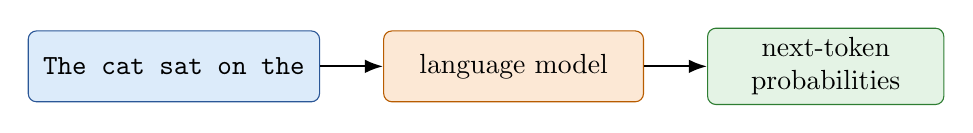
\begin{tikzpicture}[
      stage/.style={draw, rounded corners=3pt, minimum height=0.9cm,
        align=center},
      >=Latex
    ]
      \node[stage, fill=tokenblue, draw=tokenblueborder,
        minimum width=3.7cm] (context) {\texttt{The cat sat on the}};
      \node[stage, fill=tokenorange, draw=tokenorangeborder,
        right=0.8cm of context, minimum width=3.3cm] (model)
        {language model};
      \node[stage, fill=tokengreen, draw=tokengreenborder,
        right=0.8cm of model, minimum width=3.0cm] (next)
        {next-token\\probabilities};
      \draw[->, thick] (context) -- (model);
      \draw[->, thick] (model) -- (next);
    \end{tikzpicture}
  \end{center}

  \vspace{0.3em}
  \begin{columns}[T]
    \begin{column}{0.46\textwidth}
      \centering
      \begin{tabular}{lc}
        \textbf{Candidate} & \textbf{Probability} \\
        \hline
        \tokenbox[tokengreen]{mat}   & $0.46$ \\
        \tokenbox[tokengreen]{floor} & $0.21$ \\
        \tokenbox[tokengreen]{sofa}  & $0.12$ \\
        other tokens                 & $0.21$
      \end{tabular}
    \end{column}
    \begin{column}{0.50\textwidth}
      \begin{enumerate}
        \item Choose or sample one next token.
        \item Append it to the existing sequence.
        \item Feed the longer sequence back into the model.
        \item Repeat until generation stops.
      \end{enumerate}
    \end{column}
  \end{columns}

  \vfill
  \begin{alertblock}{Why begin with tokens?}
    The model generates one token at a time, so we first need to understand
    what tokens are and how text becomes a token sequence.
  \end{alertblock}
\end{frame}

\begin{frame}{A token is a discrete piece of data}
  \begin{center}
    \begin{tikzpicture}[
      item/.style={draw, rounded corners=3pt, minimum width=3.2cm,
        minimum height=2.4cm, align=center, line width=0.8pt},
      label/.style={font=\bfseries}
    ]
      \node[item, fill=tokenblue, draw=tokenblueborder] (text) {
        \textbf{Text}\\[0.4em]
        \texttt{ing}\qquad\texttt{,}\\[0.35em]
        {\scriptsize subword or punctuation}
      };
      \node[item, fill=tokenorange, draw=tokenorangeborder,
        right=0.5cm of text] (image) {
        \textbf{Image}\\[0.35em]
        \begin{tikzpicture}[scale=0.25]
          \foreach \x in {0,...,3}
            \foreach \y in {0,...,3}
              \draw[fill=white] (\x,\y) rectangle +(1,1);
          \fill[tokenorangeborder!65] (1,1) rectangle +(2,2);
          \draw[line width=1pt] (1,1) rectangle +(2,2);
        \end{tikzpicture}\\[-0.2em]
        {\scriptsize patch or visual code}
      };
      \node[item, fill=tokengreen, draw=tokengreenborder,
        right=0.5cm of image] (audio) {
        \textbf{Audio}\\[0.35em]
        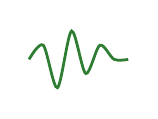
\begin{tikzpicture}[x=0.18cm,y=0.18cm]
          \draw[tokengreenborder, line width=1pt]
            plot[smooth] coordinates {(0,2) (1,3) (2,0) (3,4)
              (4,1) (5,3) (6,2) (7,2)};
        \end{tikzpicture}\\[0.25em]
        {\scriptsize short segment or codec code}
      };
    \end{tikzpicture}
  \end{center}

  \begin{block}{Common idea}
    A model processes a sequence of numbered units. The tokenizer decides
    where one unit ends and the next begins.
  \end{block}
\end{frame}

\begin{frame}{Text can be split in different ways}
  \small
  Consider the same input: \texttt{unbelievable!}

  \vspace{0.8em}
  \begin{tabular}{@{}p{2.2cm}p{8.8cm}@{}}
    \textbf{Characters} &
      \tokenbox{u}\,\tokenbox{n}\,\tokenbox{b}\,\tokenbox{e}\,
      \tokenbox{l}\,\tokenbox{i}\,\tokenbox{e}\,\tokenbox{v}\,
      \tokenbox{a}\,\tokenbox{b}\,\tokenbox{l}\,\tokenbox{e}\,
      \tokenbox{!} \\[0.8em]
    \textbf{Words} &
      \tokenbox[tokenorange]{unbelievable}\,\tokenbox[tokenorange]{!}
      \\[0.8em]
    \textbf{Subwords} &
      \tokenbox[tokengreen]{un}\,\tokenbox[tokengreen]{believ}\,
      \tokenbox[tokengreen]{able}\,\tokenbox[tokengreen]{!}
  \end{tabular}

  \vfill
  \begin{alertblock}{Why subwords?}
    Frequent strings can become one token, while rare words can still be
    assembled from smaller pieces. A token is therefore not necessarily a
    character or a complete word.
  \end{alertblock}

  {\scriptsize The subword split above is illustrative; the result depends on
  the tokenizer and its training data.}
\end{frame}

\begin{frame}{How repeated strings become tokens: toy BPE}
  \footnotesize
  \textbf{Byte Pair Encoding (BPE)} starts with characters; each word in this
  toy corpus occurs once.

  \vspace{0.15em}
  {\centering
    \tokenbox{play}\quad
    \tokenbox{played}\quad
    \tokenbox{player}\quad
    \tokenbox{playing}\par
  }

  At every round, count \emph{adjacent pairs across the whole corpus}, then
  replace one most-frequent pair with a new symbol.

  \vspace{0.2em}
  \begin{columns}[T]
    \begin{column}{0.59\textwidth}
      \centering
      {\scriptsize
      \begin{tabular}{clcl}
        \textbf{Round} & \textbf{Selected pair} & \textbf{Count} &
          \textbf{Common prefix} \\
        \hline
        0 & --                 & -- & \texttt{p l a y} \\
        1 & \texttt{p + l}    & 4  & \texttt{pl a y} \\
        2 & \texttt{pl + a}   & 4  & \texttt{pla y} \\
        3 & \texttt{pla + y}  & 4  & \texttt{play} \\
      \end{tabular}
      }

      \vspace{0.4em}
      {\scriptsize Initially several pairs tie at count 4; a fixed tie-breaking
      rule chooses which equally frequent pair is merged first.}
    \end{column}
    \begin{column}{0.37\textwidth}
      \begin{block}{What does count 4 mean?}
        The selected pair appears once in each of the four words, for four
        occurrences across the corpus.
      \end{block}

      \centering
      After round 3:\par\smallskip
      {\scriptsize
      \begin{tabular}{rcl}
        \texttt{played} & $\rightarrow$ &
          \texttt{[play][e][d]} \\
        \texttt{player} & $\rightarrow$ &
          \texttt{[play][e][r]}
      \end{tabular}
      }
    \end{column}
  \end{columns}

  \vfill
  \begin{alertblock}{Stopping criterion}
    This example stops after round 3 only to highlight \texttt{play}. Real BPE
    continues to a merge budget or target vocabulary size. Here, the next merge
    is \texttt{play + e}, which occurs twice.
  \end{alertblock}
\end{frame}

\begin{frame}{A vocabulary maps tokens to integer IDs}
  \begin{columns}[T]
    \begin{column}{0.43\textwidth}
      \centering
      \textbf{Tiny illustrative vocabulary}

      \vspace{0.5em}
      \begin{tabular}{rcl}
        \textbf{ID} & & \textbf{Token} \\
        \hline
        7   & $\leftrightarrow$ & \tokenbox[tokenorange]{!} \\
        41  & $\leftrightarrow$ & \tokenbox[tokenorange]{<space>} \\
        88  & $\leftrightarrow$ & \tokenbox[tokenorange]{er} \\
        314 & $\leftrightarrow$ & \tokenbox[tokenorange]{play} \\
      \end{tabular}
    \end{column}
    \begin{column}{0.53\textwidth}
      Input begins with a space: \texttt{player!}
      \[
        \tokenbox{<space>}\,
        \tokenbox{play}\,
        \tokenbox{er}\,
        \tokenbox{!}
      \]
      \[
        \longrightarrow [41,\,314,\,88,\,7]
      \]

      \begin{block}{IDs are labels, not quantities}
        ID 314 is not ``larger in meaning'' than ID 88. The numbers only index
        entries in a fixed list.
      \end{block}
    \end{column}
  \end{columns}

  \vfill
  \small Whitespace and punctuation also carry information. Depending on the
  tokenizer, a space may be separate or attached to a neighboring token.

  \medskip
  \begin{center}
    \textbf{The complete collection of all available tokens is the vocabulary,
    denoted $V$.}
  \end{center}
\end{frame}

% !TEX root = ../main.tex

\section{Vectors and embeddings}

\begin{frame}{Scalar, vector, matrix, tensor}
  \small
  These names describe how numbers are arranged into axes:

  \vspace{0.7em}
  \begin{tabular}{@{}p{2.0cm}p{4.7cm}p{3.9cm}@{}}
    \toprule
    \textbf{Name} & \textbf{Example} & \textbf{Rank and shape} \\
    \midrule
    Scalar & \(s=3.2\) & rank 0, shape \(()\) \\[0.65em]
    Vector & \(\mathbf{x}=\begin{bmatrix}0.2&-0.7&0.4\end{bmatrix}\)
      & rank 1, shape \((3)\) \\[0.65em]
    Matrix & \(X=\begin{bmatrix}0.2&-0.7&0.4\\0.1&0.8&-0.3\end{bmatrix}\)
      & rank 2, shape \((2,3)\) \\[0.65em]
    Tensor & \(T=\left[\begin{matrix}X_1\\X_2\\\vdots\end{matrix}\right]\)
      & rank 3, shape \((b,n,d)\) \\
    \bottomrule
  \end{tabular}

  \vfill
  \begin{block}{Terminology}
    A tensor is the general object; a scalar, vector, and matrix are rank-0,
    rank-1, and rank-2 tensors. Shape gives the size along every axis.
  \end{block}
\end{frame}

\begin{frame}{Embedding lookup: from an ID to a vector}
  \small
  Let \(|V|\) be the number of tokens. The embedding dimension \(d\) is a model
  hyperparameter: the chosen width of every token vector. The model stores the
  learnable \emph{embedding matrix} \(W_E\):
  \[
    W_E\in\mathbb{R}^{d\times |V|}.
  \]

  \begin{center}
    \begin{tikzpicture}[>=Latex]
      \node[draw=tokenblueborder, fill=tokenblue, rounded corners,
        minimum width=1.6cm, minimum height=0.8cm] (id) {ID \(i=2\)};

      \node[right=2.2cm of id] (matrix) {\(
        W_E=\begin{bmatrix}
          0.1 & \phantom{-}0.7 & \colorbox{tokengreen}{\(-0.3\)} & 0.0\\
          -0.4 & \phantom{-}0.2 &
          \colorbox{tokengreen}{\(\phantom{-}0.8\)} & -0.2\\
          0.6 & -0.1 &
          \colorbox{tokengreen}{\(\phantom{-}0.5\)} & \phantom{-}0.9
        \end{bmatrix}\)};

      \node[draw=tokengreenborder, fill=tokengreen, rounded corners,
        right=1.2cm of matrix, align=center] (vector)
        {\(\mathbf{e}_i=(W_E)_{:,i}\)\\[0.2em]
         \(=[-0.3,0.8,0.5]^{\mathsf T}\)};

      \draw[->, thick] (id) -- node[above]{select column} (matrix);
      \draw[->, thick] (matrix) -- (vector);
    \end{tikzpicture}
  \end{center}

  \begin{block}{Lookup versus learning}
    During a forward pass, lookup simply selects a column. During training,
    gradients update the values in every token column. Over many examples,
    the token vectors develop meaningful geometric relationships based on how
    the tokens are used.
  \end{block}
\end{frame}

\begin{frame}{Training learns the embedding values}
  \small
  The embedding matrix \(W_E\) is a set of model parameters. Token IDs select its
  columns, but next-token training determines the numbers stored in them.

  \vspace{0.4em}
  \begin{center}
    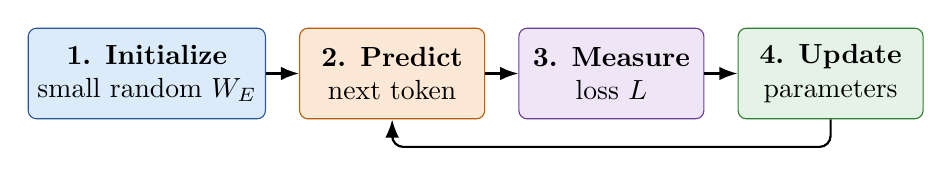
\begin{tikzpicture}[
      stage/.style={draw, rounded corners=3pt, minimum height=1.15cm,
        minimum width=2.35cm, align=center},
      >=Latex
    ]
      \node[stage, fill=tokenblue, draw=tokenblueborder] (initial)
        {\textbf{1. Initialize}\\small random \(W_E\)};
      \node[stage, fill=tokenorange, draw=tokenorangeborder,
        right=0.42cm of initial] (predict)
        {\textbf{2. Predict}\\next token};
      \node[stage, fill=tensorpurple, draw=tensorpurpleborder,
        right=0.42cm of predict] (loss)
        {\textbf{3. Measure}\\loss \(L\)};
      \node[stage, fill=tokengreen, draw=tokengreenborder,
        right=0.42cm of loss] (update)
        {\textbf{4. Update}\\parameters};
      \draw[->, thick] (initial) -- (predict);
      \draw[->, thick] (predict) -- (loss);
      \draw[->, thick] (loss) -- (update);
      \draw[->, thick, rounded corners]
        (update.south) -- ++(0,-0.35) -| (predict.south);
    \end{tikzpicture}
  \end{center}

  \begin{columns}[T]
    \begin{column}{0.47\textwidth}
      \begin{block}{Next-token loss}
        If the correct next token is \(y\), the cross-entropy contribution is
        \[
          L=-\log p(y\mid x).
        \]
        High probability for \(y\) gives a small loss; low probability gives a
        large loss.
      \end{block}
    \end{column}
    \begin{column}{0.47\textwidth}
      \begin{block}{Learning from the loss}
        Backpropagation computes \(\nabla_{W_E}L\). An optimizer with learning rate
        \(\eta{}\) updates the matrix:
        \[
          W_E\leftarrow W_E-\eta\nabla_{W_E}L.
        \]
        Repeating this loop gives the columns useful values.
      \end{block}
    \end{column}
  \end{columns}
\end{frame}

\begin{frame}{Cross-entropy strongly penalizes low probability}
  \small
  Let \(p=p(y\mid x)\) be the probability assigned to the correct next token.
  Its loss is \(L(p)=-\log p\) (using the natural logarithm).

  \begin{center}
    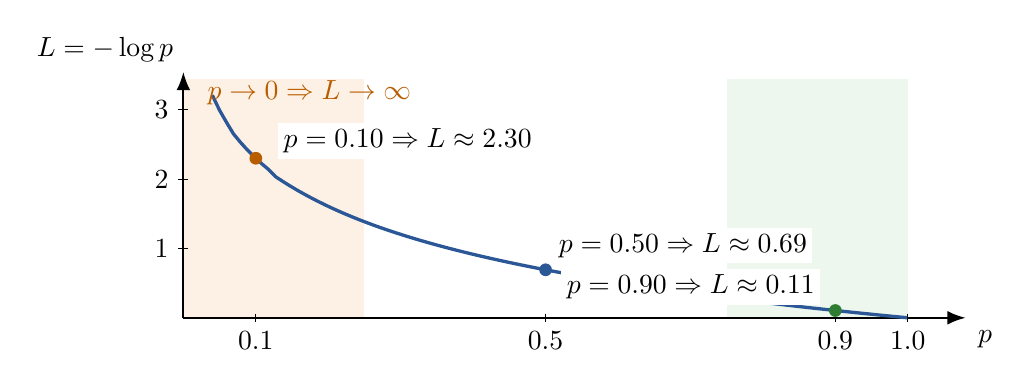
\begin{tikzpicture}[x=9.2cm, y=0.88cm, >=Latex]
      \fill[tokenorange, opacity=0.65] (0,0) rectangle (0.25,3.45);
      \fill[tokengreen, opacity=0.65] (0.75,0) rectangle (1,3.45);

      \draw[->, thick] (0,0) -- (1.08,0)
        node[below right=1pt] {\(p\)};
      \draw[->, thick] (0,0) -- (0,3.55)
        node[above left] {\(L=-\log p\)};

      \foreach \x/\label in {0.1/{0.1},0.5/{0.5},0.9/{0.9},1/{1.0}} {
        \draw (\x,0.06) -- (\x,-0.06) node[below] {\(\label\)};
      }
      \foreach \y in {1,2,3} {
        \draw (0.007,\y) -- (-0.007,\y) node[left] {\(\y\)};
      }

      \draw[very thick, tokenblueborder, domain=0.04:1, samples=100,
        variable=\p]
        plot ({\p},{-ln(\p)});

      \fill[tokenorangeborder] (0.1,2.3026) circle (2.3pt);
      \node[anchor=west, fill=white, inner sep=2pt]
        at (0.13,2.55) {\(p=0.10 \Rightarrow L\approx2.30\)};

      \fill[tokenblueborder] (0.5,0.6931) circle (2.3pt);
      \node[anchor=south west, fill=white, inner sep=2pt]
        at (0.51,0.78) {\(p=0.50 \Rightarrow L\approx0.69\)};

      \fill[tokengreenborder] (0.9,0.1054) circle (2.3pt);
      \node[anchor=south east, fill=white, inner sep=2pt]
        at (0.88,0.18) {\(p=0.90 \Rightarrow L\approx0.11\)};

      \node[tokenorangeborder, anchor=west] at (0.02,3.25)
        {\(p\to0 \Rightarrow L\to\infty\)};
    \end{tikzpicture}
  \end{center}

  \vspace{-0.15em}
  \begin{alertblock}{Training signal}
    A confident wrong prediction receives a large penalty; assigning the
    correct token probability near \(1\) drives its loss toward \(0\).
  \end{alertblock}
\end{frame}

\begin{frame}{Unembedding is needed to make predictions}
  \small
  To evaluate the loss \(L\), the model must make a next-token prediction.
  For now, treat the Transformer as a black box: it turns the input token
  vectors into a context vector \(\mathbf h\).

  \begin{center}
    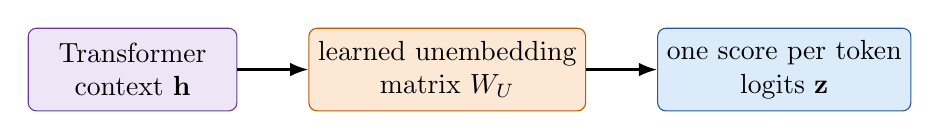
\begin{tikzpicture}[
      stage/.style={draw, rounded corners=3pt, minimum width=2.65cm,
        minimum height=1.05cm, align=center},
      >=Latex
    ]
      \node[stage, fill=tensorpurple, draw=tensorpurpleborder] (transformer)
        {Transformer\\context \(\mathbf h\)};
      \node[stage, fill=tokenorange, draw=tokenorangeborder,
        right=0.9cm of transformer] (unembed)
        {learned unembedding\\matrix \(W_U\)};
      \node[stage, fill=tokenblue, draw=tokenblueborder,
        right=0.9cm of unembed] (logits)
        {one score per token\\logits \(\mathbf z\)};
      \draw[->, thick] (transformer) -- (unembed);
      \draw[->, thick] (unembed) -- (logits);
    \end{tikzpicture}
  \end{center}

  \begin{columns}[T]
    \begin{column}{0.47\textwidth}
      \begin{block}{Embedding \(W_E\)}
        Token ID \(\longrightarrow{}\) input token vector
      \end{block}
    \end{column}
    \begin{column}{0.47\textwidth}
      \begin{block}{Unembedding \(W_U\)}
        Context vector \(\longrightarrow{}\) token scores
      \end{block}
    \end{column}
  \end{columns}

  \begin{alertblock}{Why training needs both matrices}
    \(W_E\) supplies the vectors that enter the Transformer. \(W_U\) supplies
    one candidate vector for every possible next token, letting the model
    produce the scores needed for its prediction and loss.
  \end{alertblock}
\end{frame}

\begin{frame}{Dot product: scoring a candidate token}
  \small
  Input token vectors come from columns of \(W_E\). After the Transformer has
  combined their context, candidate token \(j\) uses column
  \(\mathbf w_j={(W_U)}_{:,j}\). Its logit is the dot product
  \(z_j=\mathbf{h}^{\mathsf T}\mathbf{w}_j\).

  \begin{columns}[T]
    \begin{column}{0.41\textwidth}
      \centering
      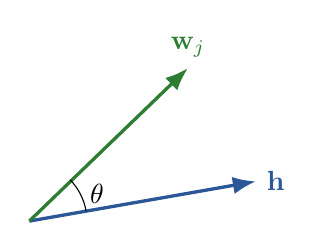
\begin{tikzpicture}[scale=0.72, >=Latex]
        \coordinate (o) at (0,0);
        \draw[->, very thick, tokenblueborder] (o) -- (4.0,0.7)
          node[right] {\(\mathbf{h}\)};
        \draw[->, very thick, tokengreenborder] (o) -- (2.8,2.7)
          node[above] {\(\mathbf{w}_j\)};
        \draw (1.0,0.18) arc[start angle=10,end angle=44,radius=1.05]
          node[midway, right] {\(\theta\)};
      \end{tikzpicture}

      \[
        \mathbf{h}^{\mathsf T}\mathbf{w}_j
        =\lVert\mathbf{h}\rVert
         \lVert\mathbf{w}_j\rVert\cos\theta
      \]
    \end{column}
    \begin{column}{0.55\textwidth}
      \footnotesize
      \begin{block}{Dot-product intuition}
        The score grows when the vectors point in similar directions, but also
        when either vector is longer.
      \end{block}

      \begin{block}{Cosine removes length}
        \[
          \cos\theta=
          \frac{\mathbf{h}^{\mathsf T}\mathbf{w}_j}
          {\lVert\mathbf{h}\rVert\lVert\mathbf{w}_j\rVert}.
        \]
        Dividing out both lengths keeps only directional similarity.
      \end{block}
    \end{column}
  \end{columns}

  \vspace{-0.2em}
  \begin{alertblock}{Connection to cross-entropy}
    \footnotesize
    Dot products produce candidate scores. Cross-entropy pushes the correct
    token's score above its competing tokens.
  \end{alertblock}
\end{frame}

\begin{frame}{From logits to probabilities: softmax}
  \small
  The model produces one raw score, or \emph{logit} \(z_j\), for every token
  \(j\in V\). Logits can be any real numbers and do not have to sum to \(1\).

  \vspace{0.3em}
  \begin{columns}[c]
    \begin{column}{0.49\textwidth}
      \centering
      \textbf{Normalize all vocabulary scores together}
      \[
        p_j=p(y=j\mid x)
        =\frac{e^{z_j}}{\displaystyle\sum_{k\in V}e^{z_k}}
      \]
    \end{column}
    \begin{column}{0.46\textwidth}
      \begin{itemize}
        \item \(e^{z_j}>0\) makes every result positive.
        \item The shared denominator makes
          \(\sum_{j\in V}p_j=1\).
        \item Larger logits receive larger probabilities.
      \end{itemize}
    \end{column}
  \end{columns}

  \begin{center}
    \footnotesize
    \renewcommand{\arraystretch}{1.12}
    \begin{tabular}{cccc}
      \toprule
      Candidate token & Logit \(z_j\) & \(e^{z_j}\) & Probability \(p_j\) \\
      \midrule
      \texttt{cat}  & \(2.0\) & \(7.39\) & \(0.67\) \\
      \texttt{dog}  & \(1.0\) & \(2.72\) & \(0.24\) \\
      \texttt{runs} & \(0.0\) & \(1.00\) & \(0.09\) \\
      \midrule
      & & \(11.11\) & \(1.00\) \\
      \bottomrule
    \end{tabular}
  \end{center}

  \vspace{-1.4em}
  \begin{alertblock}{Connecting probabilities to the loss}
    \footnotesize
    If the correct token is \texttt{cat}, then \(p_y=0.67\) and
    \(L=-\log(0.67)\approx0.40\).
  \end{alertblock}
\end{frame}

\begin{frame}{Why does \(e\) appear in softmax?}
  \small
  \begin{center}
    \large\itshape
    ``That's a great question, because the answer isn't
    \emph{'because mathematicians like \(e\)'}''.
  \end{center}

  \begin{center}
    \begin{tikzpicture}[
      stage/.style={draw, rounded corners=3pt, minimum height=1.0cm,
        minimum width=2.9cm, align=center},
      >=Latex
    ]
      \node[stage, fill=tensorpurple, draw=tensorpurpleborder] (scores)
        {logits\\\(z_j\in\mathbb R\)};
      \node[stage, fill=tokenorange, draw=tokenorangeborder,
        right=0.7cm of scores] (weights)
        {exponentiate\\\(w_j=e^{z_j}>0\)};
      \node[stage, fill=tokengreen, draw=tokengreenborder,
        right=0.7cm of weights] (probabilities)
        {normalize\\\(p_j=\dfrac{w_j}{\sum_k w_k}\)};
      \draw[->, thick] (scores) -- (weights);
      \draw[->, thick] (weights) -- (probabilities);
    \end{tikzpicture}
  \end{center}

  \vspace{-1em}
  \begin{columns}[T,onlytextwidth]
    \begin{column}{0.49\textwidth}
      \begin{block}{Why an exponential?}
        \small
        It is positive, preserves order, and a common shift cancels:
        \[
          \frac{e^{z_j+c}}{\sum_k e^{z_k+c}}
          =\frac{e^c e^{z_j}}{e^c\sum_k e^{z_k}}
          =\frac{e^{z_j}}{\sum_k e^{z_k}}.
        \]
        Only differences between logits affect the probabilities.
      \end{block}
    \end{column}
    \begin{column}{0.45\textwidth}
      \begin{block}{Why specifically base \(e\)?}
        \small
        Any base \(a>1\) could work, since
        \[
          a^z=e^{(\ln a)z}.
        \]
        The base only rescales the logits. But
        \[
          \frac{d}{dz}a^z=(\ln a)a^z,
          \qquad
          \frac{d}{dz}e^z=e^z.
        \]
        Base \(e\) removes the extra factor, keeping learning gradients clean.
      \end{block}
    \end{column}
  \end{columns}
\end{frame}

\begin{frame}{Embeddings turn usage into geometry}
  \small
  \begin{columns}[T]
    \begin{column}{0.55\textwidth}
      \centering
      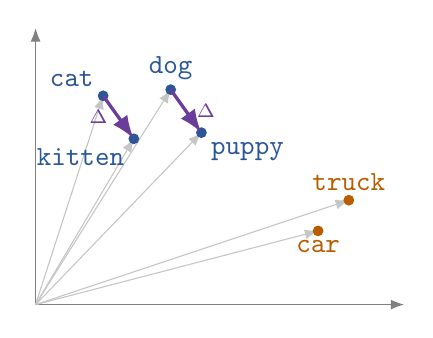
\begin{tikzpicture}[scale=0.78, >=Latex]
        \draw[->, gray] (0,0) -- (6.0,0);
        \draw[->, gray] (0,0) -- (0,4.5);

        \foreach \point in {
          (1.1,3.4),(2.2,3.5),(1.6,2.7),(2.7,2.8),
          (4.6,1.2),(5.1,1.7)
        } {
          \draw[->, thin, gray!45] (0,0) -- \point;
        }

        \fill[tokenblueborder] (1.1,3.4) circle (2.5pt)
          node[above left]{\texttt{cat}};
        \fill[tokenblueborder] (2.2,3.5) circle (2.5pt)
          node[above]{\texttt{dog}};
        \fill[tokenblueborder] (1.6,2.7) circle (2.5pt)
          node[below left]{\texttt{kitten}};
        \fill[tokenblueborder] (2.7,2.8) circle (2.5pt)
          node[below right]{\texttt{puppy}};

        \draw[->, very thick, tensorpurpleborder] (1.1,3.4) -- (1.6,2.7)
          node[midway, left, font=\scriptsize] {\(\Delta\)};
        \draw[->, very thick, tensorpurpleborder] (2.2,3.5) -- (2.7,2.8)
          node[midway, right, font=\scriptsize] {\(\Delta\)};

        \fill[tokenorangeborder] (4.6,1.2) circle (2.5pt)
          node[below]{\texttt{car}};
        \fill[tokenorangeborder] (5.1,1.7) circle (2.5pt)
          node[above]{\texttt{truck}};

      \end{tikzpicture}

      \vspace{-0.3em}
      {\scriptsize
      \(
        \begin{aligned}
          \mathbf{e}_{\text{puppy}}-\mathbf{e}_{\text{dog}}
            &\approx \boldsymbol{\Delta},\\
          \mathbf{e}_{\text{kitten}}-\mathbf{e}_{\text{cat}}
            &\approx \boldsymbol{\Delta}.
        \end{aligned}
      \)}

      \smallskip
      \textbf{Both arrows show the same relative move:}
      adult animal \(\rightarrow{}\) young animal.
    \end{column}
    \begin{column}{0.42\textwidth}
      Tokens used in similar contexts often acquire related locations.

      \vspace{0.8em}
      Cosine similarity measures directional similarity:
      \[
        \cos(\mathbf{a},\mathbf{b})=
        \frac{\mathbf{a}\cdot\mathbf{b}}
        {\lVert\mathbf{a}\rVert\lVert\mathbf{b}\rVert}.
      \]

    \end{column}
  \end{columns}

  \vspace{-0.3em}
  \begin{alertblock}{Measure, not objective}
    \footnotesize
    Next-token cross-entropy is the training objective; cosine similarity only
    inspects learned geometry. Lookup embeddings are static; contextual
    representations come later.
  \end{alertblock}
\end{frame}

\begin{frame}{Scale example: the GPT-3 175B embedding matrix}
  \small
  The largest GPT-3 model uses a vocabulary of \(50{,}257\) tokens and an
  embedding dimension of \(d=12{,}288\).

  \[
    W_E\in\mathbb R^{12{,}288\times 50{,}257}
    \qquad
    \text{(\(d\) rows, one column per token).}
  \]

  \begin{center}
    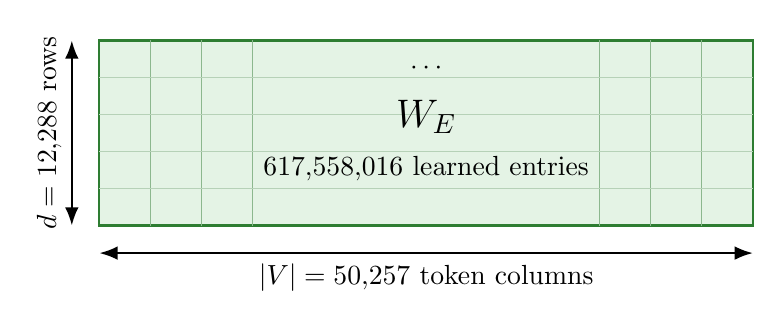
\begin{tikzpicture}[>=Latex]
      \fill[tokengreen] (0,0) rectangle (8.3,2.35);
      \draw[tokengreenborder, thick] (0,0) rectangle (8.3,2.35);

      \foreach \x in {0.65,1.3,1.95,6.35,7.0,7.65} {
        \draw[tokengreenborder!55] (\x,0) -- (\x,2.35);
      }
      \foreach \y in {0.47,0.94,1.41,1.88} {
        \draw[tokengreenborder!35] (0,\y) -- (8.3,\y);
      }

      \node[font=\Large] at (4.15,1.38) {\(W_E\)};
      \node at (4.15,0.72) {\(617{,}558{,}016\) learned entries};
      \node at (4.15,2.0) {\(\cdots\)};

      \draw[<->, thick] (0,-0.35) -- (8.3,-0.35)
        node[midway, below] {\(|V|=50{,}257\) token columns};
      \draw[<->, thick] (-0.35,0) -- (-0.35,2.35)
        node[midway, above, rotate=90] {\(d=12{,}288\) rows};
    \end{tikzpicture}
  \end{center}

  \vspace{-0.65em}
  \begin{alertblock}{Parameter count and matching dimensions}
    \footnotesize
    \centering
    \(50{,}257\times12{,}288
      =\boxed{617{,}558{,}016}\approx 618\text{ million parameters}\).

    \smallskip
    For GPT-3, \(W_U\) has the same shape as \(W_E\):
    \(W_U,W_E\in\mathbb R^{12{,}288\times50{,}257}\).
    Equal shape does not mean equal entries.
  \end{alertblock}
\end{frame}

\begin{frame}[plain]
  \centering
  \vfill

  {\Huge Short break}

  \vspace{1.2em}
  {\large Tokens \(\rightarrow{}\) IDs \(\rightarrow{}\) embeddings \(\rightarrow{}\)
  next-token loss \quad \checkmark}

  \vspace{2.0em}
  {\Large Next: inside the Transformer}

  \vspace{0.5em}
  {\normalsize How do token representations exchange context?}

  \vfill
\end{frame}

\begin{frame}{A token sequence becomes a matrix}
  \small
  \begin{center}
    \tokenbox{the}\quad\tokenbox{cat}\quad\tokenbox{sleeps}
    \(\quad\longrightarrow\quad{}\)
    \([12,51,908]\)
  \end{center}

  \vspace{0.3em}
  Each ID selects one column from \(W_E\). Stacking the transposed vectors gives
  \[
    X=
    \begin{bmatrix}
      \mathbf{e}_{12}^{\mathsf T}\\
      \mathbf{e}_{51}^{\mathsf T}\\
      \mathbf{e}_{908}^{\mathsf T}
    \end{bmatrix}
    \in\mathbb{R}^{n\times d},
    \qquad n=3.
  \]

  \begin{center}
    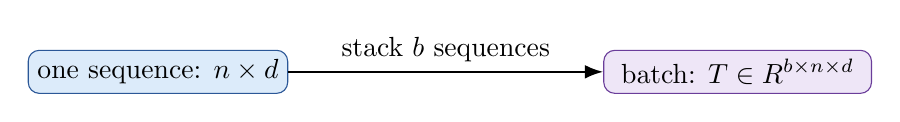
\begin{tikzpicture}[>=Latex, node distance=0.55cm]
      \node[draw=tokenblueborder, fill=tokenblue, rounded corners,
        minimum width=3.1cm] (sequence) {one sequence: \(n\times d\)};
      \node[draw=tensorpurpleborder, fill=tensorpurple, rounded corners,
        right=4.0cm of sequence, minimum width=3.4cm] (batch)
        {batch: \(T\in\mathbb{R}^{b\times n\times d}\)};
      \draw[->, thick] (sequence) -- node[above]{stack \(b\) sequences} (batch);
    \end{tikzpicture}
  \end{center}

  {\scriptsize Sequences in a batch are commonly padded to a shared length;
  a mask tells later layers which positions are padding.}
\end{frame}

\section{Transformers and attention}

\begin{frame}{From token vectors to contextual vectors}
  \begin{center}
    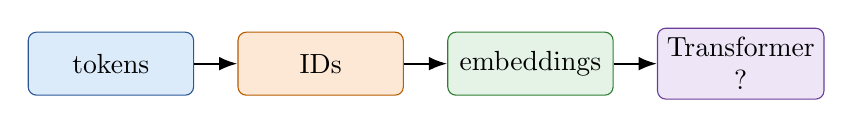
\begin{tikzpicture}[
      stage/.style={draw, rounded corners=3pt, minimum width=2.1cm,
        minimum height=0.8cm, align=center},
      >=Latex
    ]
      \node[stage, fill=tokenblue, draw=tokenblueborder] (tokens) {tokens};
      \node[stage, fill=tokenorange, draw=tokenorangeborder,
        right=0.55cm of tokens] (ids) {IDs};
      \node[stage, fill=tokengreen, draw=tokengreenborder,
        right=0.55cm of ids] (vectors) {embeddings};
      \node[stage, fill=tensorpurple, draw=tensorpurpleborder,
        right=0.55cm of vectors] (transformer) {Transformer\\?};
      \draw[->, thick] (tokens) -- (ids);
      \draw[->, thick] (ids) -- (vectors);
      \draw[->, thick] (vectors) -- (transformer);
    \end{tikzpicture}
  \end{center}

  \vspace{0.8em}
  The embedding lookup gives \tokenbox{bank} the same starting vector in both
  sentences:
  \begin{itemize}
    \item ``They sat on the river \textbf{bank}''.
    \item ``She deposited money at the \textbf{bank}''.
  \end{itemize}

  \begin{alertblock}{The problem self-attention solves}
    How can every token exchange information with the other tokens so that its
    vector reflects the surrounding context? The following slides build the
    mathematical mechanism that makes this possible.
  \end{alertblock}
\end{frame}

% !TEX root = ../main.tex

\section{Transformers and attention}\label{sec:attention}

\begin{frame}{From token vectors to contextual vectors}
  \begin{center}
    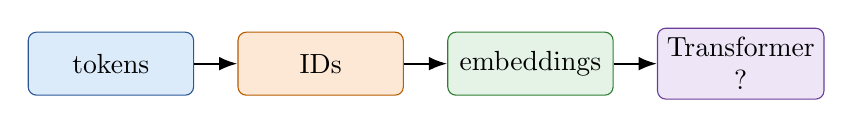
\begin{tikzpicture}[
      stage/.style={draw, rounded corners=3pt, minimum width=2.1cm,
        minimum height=0.8cm, align=center},
      >=Latex
    ]
      \node[stage, fill=tokenblue, draw=tokenblueborder] (tokens) {tokens};
      \node[stage, fill=tokenorange, draw=tokenorangeborder,
        right=0.55cm of tokens] (ids) {IDs};
      \node[stage, fill=tokengreen, draw=tokengreenborder,
        right=0.55cm of ids] (vectors) {embeddings};
      \node[stage, fill=tensorpurple, draw=tensorpurpleborder,
        right=0.55cm of vectors] (transformer) {Transformer\\?};
      \draw[->, thick] (tokens) -- (ids);
      \draw[->, thick] (ids) -- (vectors);
      \draw[->, thick] (vectors) -- (transformer);
    \end{tikzpicture}
  \end{center}

  \vspace{0.8em}
  The embedding lookup gives \tokenbox{bank} the same starting vector in both
  sentences:
  \begin{itemize}
    \item ``They sat on the river \textbf{bank}''.
    \item ``She deposited money at the \textbf{bank}''.
  \end{itemize}

  \begin{alertblock}{The problem self-attention solves}
    How can every token exchange information with the other tokens so that its
    vector reflects the surrounding context? The following slides build the
    mathematical mechanism that makes this possible.
  \end{alertblock}
\end{frame}

\begin{frame}{Attention creates a context-dependent update
  \hfill{\tiny \texttt{Head.forward}: lines 15--31}}
  \small
  The lookup vector for \texttt{bank} starts identically in both sentences.
  Attention lets it collect different clues from the surrounding tokens; we
  denote the resulting contextual vector by $\mathbf h$.

  \begin{columns}[T]
    \begin{column}{0.48\textwidth}
      \begin{block}{River context}
        \centering
        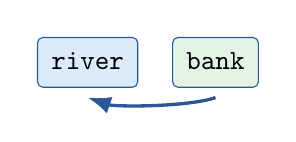
\begin{tikzpicture}[>=Latex, node distance=0.18cm]
          \node (river) {\tokenbox{river}};
          \node[right=of river] (bank) {\tokenbox[tokengreen]{bank}};
          \draw[->, very thick, tokenblueborder]
            (bank.south) .. controls +(-0.35,-0.12) and +(0.35,-0.12) ..
            (river.south);
        \end{tikzpicture}

        \[
          \mathbf e_{\text{bank}}
          \longrightarrow
          \mathbf h_{\text{bank}}^{(\text{river})}
        \]
        The result incorporates information associated with a river edge.
      \end{block}
    \end{column}
    \begin{column}{0.48\textwidth}
      \begin{block}{Financial context}
        \centering
        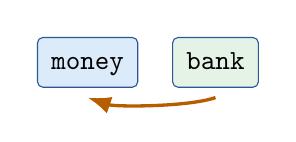
\begin{tikzpicture}[>=Latex, node distance=0.18cm]
          \node (money) {\tokenbox{money}};
          \node[right=of money] (bank) {\tokenbox[tokengreen]{bank}};
          \draw[->, very thick, tokenorangeborder]
            (bank.south) .. controls +(-0.35,-0.12) and +(0.35,-0.12) ..
            (money.south);
        \end{tikzpicture}

        \[
          \mathbf e_{\text{bank}}
          \longrightarrow
          \mathbf h_{\text{bank}}^{(\text{money})}
        \]
        The result incorporates information associated with finance.
      \end{block}
    \end{column}
  \end{columns}

  \vspace{-0.4em}
  \begin{alertblock}{The central idea}
    \footnotesize
    Each position asks which other positions matter, then mixes information
    from them. The resulting vector is contextual rather than a static lookup.
  \end{alertblock}
\end{frame}

\begin{frame}{Before attention: the model needs token order
  \hfill{\tiny \texttt{BigramLanguageModel.forward}: lines 18--23}}
  \small
  A sentence is not merely a bag of tokens: changing the order changes the
  meaning. A basic construction adds a position vector to every token vector:
  \[
    \mathbf x_i=\mathbf e_{\text{token}_i}+\mathbf p_i,
    \qquad X\in\mathbb R^{n\times d}.
  \]

  \begin{center}
    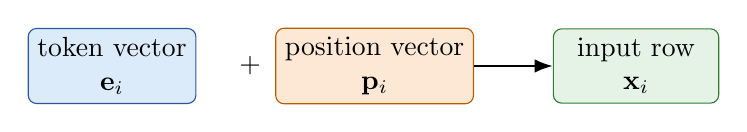
\begin{tikzpicture}[
      box/.style={draw, rounded corners=3pt, minimum width=2.1cm,
        minimum height=0.75cm, align=center},
      >=Latex
    ]
      \node[box, fill=tokenblue, draw=tokenblueborder] (token)
        {token vector\\$\mathbf e_i$};
      \node[box, fill=tokenorange, draw=tokenorangeborder,
        right=1.0cm of token] (position) {position vector\\$\mathbf p_i$};
      \node[right=0.42cm of token] (plus) {$+$};
      \node[box, fill=tokengreen, draw=tokengreenborder,
        right=1.0cm of position] (input) {input row\\$\mathbf x_i$};
      \draw[->, thick] (position) -- (input);
    \end{tikzpicture}
  \end{center}

  \begin{block}{Implementations differ}
    Position information may be learned or fixed. Rotary position encodings
    instead inject relative position when queries and keys are compared. The
    shared goal is the same: make order available to attention.
  \end{block}
\end{frame}

\begin{frame}{Query, key, value: three roles for each token
  \hfill{\tiny \texttt{Head}: lines 8--10, 17--30}}
  \small
  Self-attention derives three vectors from every input position.

  \begin{center}
    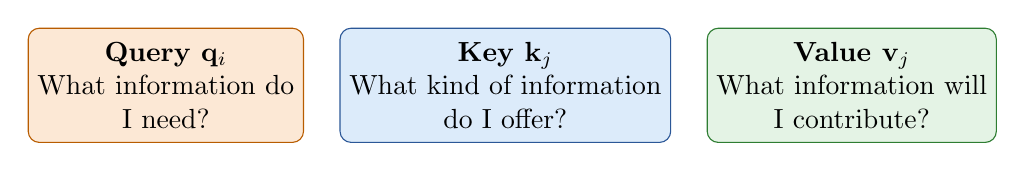
\begin{tikzpicture}[
      role/.style={draw, rounded corners=4pt, minimum width=3.35cm,
        minimum height=1.45cm, align=center},
      >=Latex
    ]
      \node[role, fill=tokenorange, draw=tokenorangeborder] (query)
        {\textbf{Query $\mathbf q_i$}\\What information do\\I need?};
      \node[role, fill=tokenblue, draw=tokenblueborder,
        right=0.45cm of query] (key)
        {\textbf{Key $\mathbf k_j$}\\What kind of information\\do I offer?};
      \node[role, fill=tokengreen, draw=tokengreenborder,
        right=0.45cm of key] (value)
        {\textbf{Value $\mathbf v_j$}\\What information will\\I contribute?};
    \end{tikzpicture}
  \end{center}

  \vspace{0.6em}
  For position $i$:
  \begin{enumerate}
    \item compare its query $\mathbf q_i$ with every allowed key $\mathbf k_j$;
    \item turn the comparison scores into attention weights;
    \item use those weights to combine the value vectors $\mathbf v_j$.
  \end{enumerate}

  \begin{alertblock}{Why ``self''-attention?}
    Queries, keys, and values all come from the same sequence $X$.
  \end{alertblock}
\end{frame}

\begin{frame}{Queries, keys, and values are learned projections
  \hfill{\tiny \texttt{Head}: lines 8--10, 17--18, 29}}
  \small
  Three learned matrices give each input row three different roles:
  \[
    Q=XW_Q,\qquad K=XW_K,\qquad V=XW_V.
  \]

  \begin{center}
    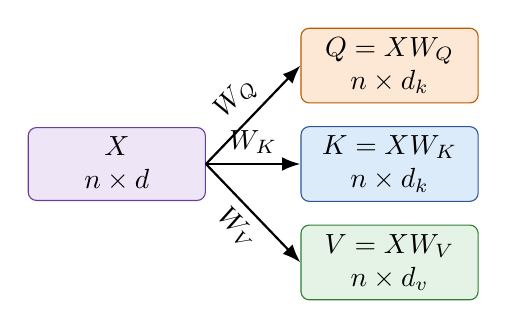
\begin{tikzpicture}[
      matrixbox/.style={draw, rounded corners=3pt, minimum height=0.9cm,
        minimum width=2.25cm, align=center},
      >=Latex
    ]
      \node[matrixbox, fill=tensorpurple, draw=tensorpurpleborder] (x)
        {$X$\\$n\times d$};
      \node[matrixbox, fill=tokenorange, draw=tokenorangeborder,
        right=1.2cm of x, yshift=1.25cm] (q) {$Q=XW_Q$\\$n\times d_k$};
      \node[matrixbox, fill=tokenblue, draw=tokenblueborder,
        right=1.2cm of x] (k) {$K=XW_K$\\$n\times d_k$};
      \node[matrixbox, fill=tokengreen, draw=tokengreenborder,
        right=1.2cm of x, yshift=-1.25cm] (v) {$V=XW_V$\\$n\times d_v$};
      \draw[->, thick] (x.east) -- (q.west)
        node[midway, above, sloped] {$W_Q$};
      \draw[->, thick] (x.east) -- (k.west)
        node[midway, above] {$W_K$};
      \draw[->, thick] (x.east) -- (v.west)
        node[midway, below, sloped] {$W_V$};
    \end{tikzpicture}
  \end{center}

  \vspace{-0.35em}
  \begin{columns}[T]
    \begin{column}{0.52\textwidth}
      \begin{block}{Shapes}
        \scriptsize
        \textbf{Weights:}
        $W_Q,W_K\in\mathbb R^{d\times d_k}$,
        $W_V\in\mathbb R^{d\times d_v}$.

        \textbf{Outputs:}
        $Q,K\in\mathbb R^{n\times d_k}$,
        $V\in\mathbb R^{n\times d_v}$.
      \end{block}
    \end{column}
    \begin{column}{0.44\textwidth}
      \begin{alertblock}{How are they learned?}
        \scriptsize
        There are no separate query, key, or value targets. Next-token
        cross-entropy backpropagates through attention and updates
        $W_Q,W_K,W_V$ with all other model weights.
      \end{alertblock}
    \end{column}
  \end{columns}
\end{frame}

\begin{frame}{Step 1: compare one query with every key
  \hfill{\tiny \texttt{Head.forward}: lines 20--22}}
  \small
  Suppose position $i$ contains \texttt{bank}. Its compatibility with an
  allowed position $j$ is the scaled dot product
  \[
    s_{ij}=\frac{\mathbf q_i^{\mathsf T}\mathbf k_j}{\sqrt{d_k}}.
  \]

  \begin{center}
    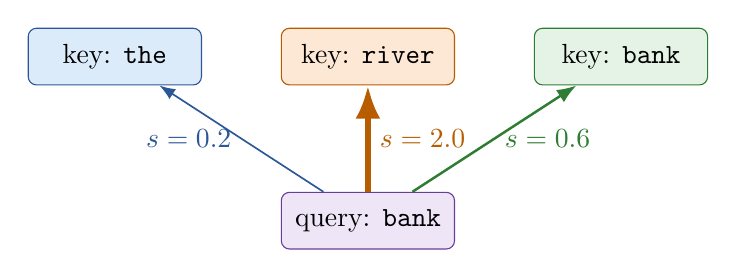
\begin{tikzpicture}[
      key/.style={draw, rounded corners=3pt, minimum width=2.2cm,
        minimum height=0.72cm, align=center},
      >=Latex
    ]
      \node[key, fill=tokenblue, draw=tokenblueborder] (the)
        {key: \texttt{the}};
      \node[key, fill=tokenorange, draw=tokenorangeborder,
        right=1.0cm of the] (river) {key: \texttt{river}};
      \node[key, fill=tokengreen, draw=tokengreenborder,
        right=1.0cm of river] (bankkey) {key: \texttt{bank}};
      \node[key, fill=tensorpurple, draw=tensorpurpleborder,
        below=1.35cm of river] (bankquery) {query: \texttt{bank}};

      \draw[->, tokenblueborder, line width=0.6pt] (bankquery) --
        node[midway, left] {$s=0.2$} (the);
      \draw[->, tokenorangeborder, line width=2.0pt] (bankquery) --
        node[midway, right] {$s=2.0$} (river);
      \draw[->, tokengreenborder, line width=0.9pt] (bankquery) --
        node[midway, right] {$s=0.6$} (bankkey);
    \end{tikzpicture}
  \end{center}

  \begin{columns}[T]
    \begin{column}{0.48\textwidth}
      \begin{block}{Interpretation}
        A larger score means the query and key are more compatible. A score is
        still an unrestricted number, not a probability.
      \end{block}
    \end{column}
    \begin{column}{0.48\textwidth}
      \begin{block}{Why divide by $\sqrt{d_k}$?}
        Dot products tend to grow as vectors get wider. Scaling keeps scores in
        a range where softmax remains responsive.
      \end{block}
    \end{column}
  \end{columns}
\end{frame}

\begin{frame}{A causal mask prevents looking into the future
  \hfill{\tiny \texttt{Head}: lines 11, 23--25}}
  \small
  During next-token prediction, position $i$ may use only positions
  $j\le i$. Forbidden scores are replaced by $-\infty$ before softmax.

  \begin{columns}[c]
    \begin{column}{0.50\textwidth}
      \[
        S=\frac{QK^{\mathsf T}}{\sqrt{d_k}}+M,
        \qquad
        M_{ij}=\begin{cases}
          0 & j\le i,\\
          -\infty & j>i.
        \end{cases}
      \]
      Because $e^{-\infty}=0$, a masked position receives zero attention
      weight.
    \end{column}
    \begin{column}{0.46\textwidth}
      \centering
      \textbf{Rows attend to columns}

      \vspace{0.4em}
      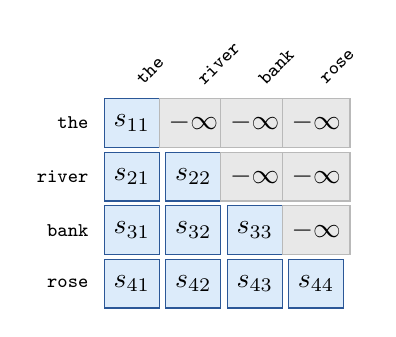
\begin{tikzpicture}[x=0.78cm,y=0.68cm]
        \foreach \r in {1,...,4} {
          \foreach \c in {1,...,4} {
            \ifnum\c>\r
              \node[draw=gray!55, fill=gray!18, minimum size=0.62cm]
                at (\c,-\r) {$-\infty$};
            \else
              \node[draw=tokenblueborder, fill=tokenblue, minimum size=0.62cm]
                at (\c,-\r) {$s_{\r\c}$};
            \fi
          }
        }
        \foreach \i/\t in {1/the,2/river,3/bank,4/rose} {
          \node[font=\scriptsize, rotate=45, anchor=west] at (\i,-0.35)
            {\texttt{\t}};
          \node[font=\scriptsize, anchor=east] at (0.45,-\i)
            {\texttt{\t}};
        }
      \end{tikzpicture}
    \end{column}
  \end{columns}

  \begin{alertblock}{No information leakage}
    The representation at position $i$ uses tokens $1,\ldots,i$ to predict
    token $i+1$. It cannot depend on token $i+1$ or anything after it.
  \end{alertblock}
\end{frame}

\begin{frame}{Step 2: softmax turns scores into attention weights
  \hfill{\tiny \texttt{Head.forward}: lines 26--27}}
  \small
  For a fixed query position $i$, normalize its allowed scores across $j$:
  \[
    \alpha_{ij}=\frac{e^{s_{ij}}}{\sum_{\ell\le i}e^{s_{i\ell}}},
    \qquad \alpha_{ij}>0,
    \qquad \sum_{j\le i}\alpha_{ij}=1.
  \]

  \begin{center}
    \renewcommand{\arraystretch}{1.25}
    \begin{tabular}{c|c|c|c}
      Key token & Score $s_{ij}$ & $e^{s_{ij}}$ & Weight $\alpha_{ij}$ \\
      \hline
      \texttt{the}   & $0.2$ & $1.22$ & $0.12$ \\
      \texttt{river} & $2.0$ & $7.39$ & $0.71$ \\
      \texttt{bank}  & $0.6$ & $1.82$ & $0.17$ \\
      \texttt{rose}  & $-\infty$ & $0$ & $0$ \\
      \hline
      & & $10.43$ & $1.00$
    \end{tabular}
  \end{center}

  \begin{alertblock}{What the weights say}
    For this illustrative head, \texttt{bank} assigns most of its attention to
    \texttt{river}. Softmax makes the comparison relative: all allowed tokens
    compete for a fixed total weight of $1$.
  \end{alertblock}
\end{frame}

\begin{frame}{Step 3: combine values into contextual information
  \hfill{\tiny \texttt{Head.forward}: lines 29--30}}
  \small
  The weights decide how much of every value vector reaches position $i$:
  \[
    \mathbf z_i=\sum_{j\le i}\alpha_{ij}\mathbf v_j.
  \]

  \begin{center}
    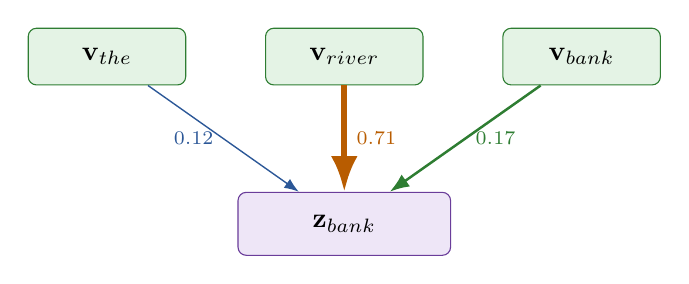
\begin{tikzpicture}[
      value/.style={draw, rounded corners=3pt, minimum width=2.0cm,
        minimum height=0.72cm, fill=tokengreen, draw=tokengreenborder},
      >=Latex
    ]
      \node[value] (the) {$\mathbf v_{\text{the}}$};
      \node[value, right=1.0cm of the] (river) {$\mathbf v_{\text{river}}$};
      \node[value, right=1.0cm of river] (bank) {$\mathbf v_{\text{bank}}$};
      \node[draw=tensorpurpleborder, fill=tensorpurple, rounded corners=3pt,
        below=1.35cm of river, minimum width=2.7cm, minimum height=0.8cm]
        (output) {$\mathbf z_{\text{bank}}$};

      \draw[->, line width=0.5pt, tokenblueborder] (the) --
        node[left, font=\scriptsize] {$0.12$} (output);
      \draw[->, line width=2.2pt, tokenorangeborder] (river) --
        node[right, font=\scriptsize] {$0.71$} (output);
      \draw[->, line width=0.9pt, tokengreenborder] (bank) --
        node[right, font=\scriptsize] {$0.17$} (output);
    \end{tikzpicture}
  \end{center}

  \[
    \mathbf z_{\text{bank}}
    =0.12\mathbf v_{\text{the}}
     +0.71\mathbf v_{\text{river}}
     +0.17\mathbf v_{\text{bank}}.
  \]

  \vspace{-0.7em}
  \begin{alertblock}{The context has entered the vector}
    \footnotesize
    The update for \texttt{bank} now contains substantial information from
    \texttt{river}. Different contexts yield different weights and therefore
    different updates.
  \end{alertblock}
\end{frame}

\begin{frame}{All positions at once: the attention equation
  \hfill{\tiny \texttt{Head.forward}: lines 17--30}}
  \small
  The per-token operations combine into one matrix expression:
  \[
    \boxed{\operatorname{Attention}(Q,K,V)
      =\operatorname{softmax}\!\left(
        \frac{QK^{\mathsf T}}{\sqrt{d_k}}+M
      \right)V}
  \]

  \begin{center}
    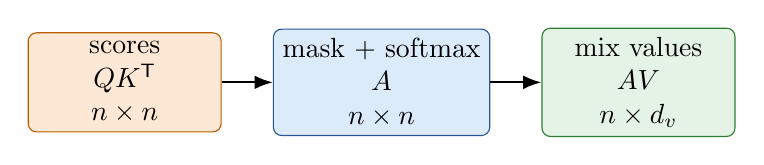
\begin{tikzpicture}[
      stage/.style={draw, rounded corners=3pt, minimum width=2.45cm,
        minimum height=1.0cm, align=center},
      >=Latex
    ]
      \node[stage, fill=tokenorange, draw=tokenorangeborder] (scores)
        {scores\\$QK^{\mathsf T}$\\$n\times n$};
      \node[stage, fill=tokenblue, draw=tokenblueborder,
        right=0.65cm of scores] (weights)
        {mask + softmax\\$A$\\$n\times n$};
      \node[stage, fill=tokengreen, draw=tokengreenborder,
        right=0.65cm of weights] (values)
        {mix values\\$AV$\\$n\times d_v$};
      \draw[->, thick] (scores) -- (weights);
      \draw[->, thick] (weights) -- (values);
    \end{tikzpicture}
  \end{center}

  \begin{block}{Reading the shape}
    The $n\times n$ matrix $A$ contains one attention distribution per row.
    Multiplying by $V$ produces one contextual update for every position.
  \end{block}
\end{frame}

\begin{frame}{Multi-head attention learns several relationships
  \hfill{\tiny \texttt{MultiHeadAttention}: lines 34--46}}
  \small
  One attention pattern need not capture every useful relationship. A
  Transformer runs $H$ attention heads with separate learned projections.

  \begin{center}
    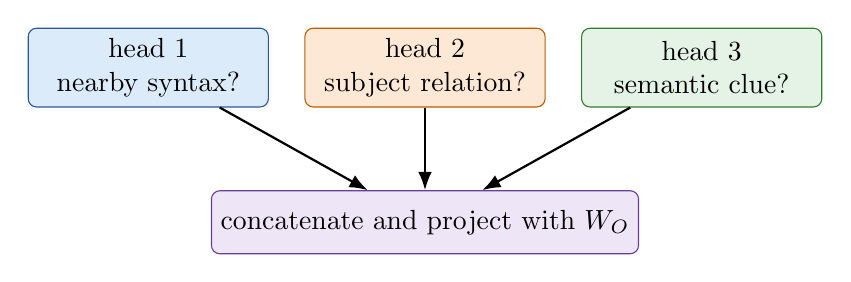
\begin{tikzpicture}[
      head/.style={draw, rounded corners=3pt, minimum width=3.05cm,
        minimum height=1.0cm, align=center},
      >=Latex
    ]
      \node[head, fill=tokenblue, draw=tokenblueborder] (h1)
        {head 1\\nearby syntax?};
      \node[head, fill=tokenorange, draw=tokenorangeborder,
        right=0.45cm of h1] (h2) {head 2\\subject relation?};
      \node[head, fill=tokengreen, draw=tokengreenborder,
        right=0.45cm of h2] (h3) {head 3\\semantic clue?};
      \node[draw=tensorpurpleborder, fill=tensorpurple, rounded corners=3pt,
        below=1.05cm of h2, minimum width=4.0cm, minimum height=0.8cm]
        (combine) {concatenate and project with $W_O$};
      \draw[->, thick] (h1) -- (combine);
      \draw[->, thick] (h2) -- (combine);
      \draw[->, thick] (h3) -- (combine);
    \end{tikzpicture}
  \end{center}

  \[
    \operatorname{MultiHead}(X)
      =\operatorname{Concat}(\text{head}_1,\ldots,\text{head}_H)W_O.
  \]

  \begin{alertblock}{Interpret the labels as intuition}
    Heads are not assigned these jobs by hand; training learns their behavior,
    and real heads may mix several kinds of relationships.
  \end{alertblock}
\end{frame}

\begin{frame}{Attention is the communication step in a Transformer block}
  \small
  \begin{center}
    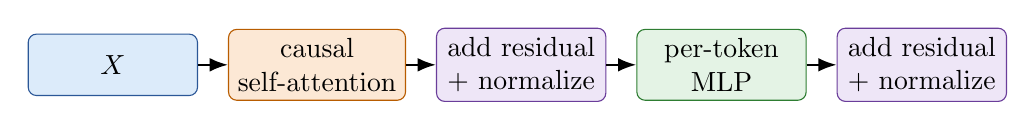
\begin{tikzpicture}[
      stage/.style={draw, rounded corners=3pt, minimum width=2.15cm,
        minimum height=0.78cm, align=center},
      >=Latex
    ]
      \node[stage, fill=tokenblue, draw=tokenblueborder] (input) {$X$};
      \node[stage, fill=tokenorange, draw=tokenorangeborder,
        right=0.38cm of input] (attention) {causal\\self-attention};
      \node[stage, fill=tensorpurple, draw=tensorpurpleborder,
        right=0.38cm of attention] (res1) {add residual\\+ normalize};
      \node[stage, fill=tokengreen, draw=tokengreenborder,
        right=0.38cm of res1] (mlp) {per-token\\MLP};
      \node[stage, fill=tensorpurple, draw=tensorpurpleborder,
        right=0.38cm of mlp] (res2) {add residual\\+ normalize};
      \draw[->, thick] (input) -- (attention);
      \draw[->, thick] (attention) -- (res1);
      \draw[->, thick] (res1) -- (mlp);
      \draw[->, thick] (mlp) -- (res2);
    \end{tikzpicture}
  \end{center}

  \vspace{0.8em}
  \begin{columns}[T]
    \begin{column}{0.48\textwidth}
      \begin{block}{Across positions}
        Self-attention moves information between tokens. The causal mask
        preserves next-token prediction.
      \end{block}
    \end{column}
    \begin{column}{0.48\textwidth}
      \begin{block}{Within each position}
        The MLP transforms each token vector independently. Residual paths help
        preserve and refine existing information.
      \end{block}
    \end{column}
  \end{columns}

  \begin{alertblock}{Depth builds richer context}
    Stacking many blocks lets information travel and be transformed repeatedly,
    producing the contextual representations used to predict the next token.
  \end{alertblock}
\end{frame}

\begin{frame}{Inside the per-token MLP: factual associations}
  \small
  \begin{center}
    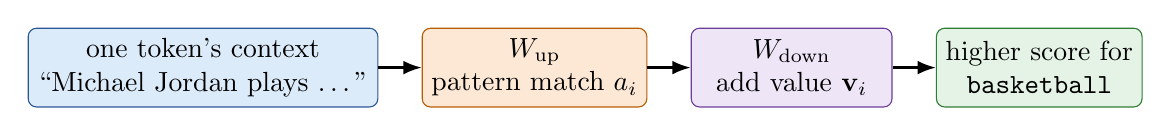
\begin{tikzpicture}[
      stage/.style={draw, rounded corners=3pt, minimum height=1.0cm,
        minimum width=2.55cm, align=center},
      >=Latex
    ]
      \node[stage, fill=tokenblue, draw=tokenblueborder] (context)
        {one token's context\\``Michael Jordan plays \ldots{}''};
      \node[stage, fill=tokenorange, draw=tokenorangeborder,
        right=0.55cm of context] (key)
        {\(W_{\mathrm{up}}\)\\pattern match \(a_i\)};
      \node[stage, fill=tensorpurple, draw=tensorpurpleborder,
        right=0.55cm of key] (value)
        {\(W_{\mathrm{down}}\)\\add value \(\mathbf v_i\)};
      \node[stage, fill=tokengreen, draw=tokengreenborder,
        right=0.55cm of value] (prediction)
        {higher score for\\\texttt{basketball}};
      \draw[->, thick] (context) -- (key);
      \draw[->, thick] (key) -- (value);
      \draw[->, thick] (value) -- (prediction);
    \end{tikzpicture}
  \end{center}

  \vspace{-0.5em}
  \[
    \operatorname{MLP}(\mathbf x)
      =\sigma(\mathbf xW_{\mathrm{up}})W_{\mathrm{down}}
      =\sum_i a_i\mathbf v_i,
    \qquad
    a_i=\sigma(\mathbf x\mathbf k_i).
  \]
  \vspace{-1.0em}
  \begin{center}
    \scriptsize
    \(\mathbf k_i\) is column \(i\) of \(W_{\mathrm{up}}\);
    \(\mathbf v_i\) is row \(i\) of \(W_{\mathrm{down}}\).
  \end{center}

  \vspace{-0.4em}
  \begin{columns}[T,onlytextwidth]
    \begin{column}{0.49\textwidth}
      \begin{block}{Geva et al. (2021)}
        \scriptsize
        \href{https://arxiv.org/abs/2012.14913}{\emph{Transformer Feed-Forward
        Layers Are Key-Value Memories}.}
        They found that \(W_{\mathrm{up}}\) directions respond to interpretable
        textual patterns, while corresponding \(W_{\mathrm{down}}\) values favor
        plausible output tokens.
      \end{block}
    \end{column}
    \begin{column}{0.49\textwidth}
      \begin{block}{Meng et al. (2022): ROME}
        \scriptsize
        \href{https://arxiv.org/abs/2202.05262}{\emph{Locating and Editing
        Factual Associations in GPT}.}
        Causal tracing localized factual predictions to middle-layer MLPs;
        rank-one changes to their feed-forward weights could update particular
        factual associations.
      \end{block}
    \end{column}
  \end{columns}

  \vspace{-0.4em}
  \begin{alertblock}{Important nuance}
    \footnotesize
    ``Michael Jordan plays basketball'' is illustrative. Evidence points to
    distributed, compositional storage---not one complete sentence in one neuron.
  \end{alertblock}
\end{frame}

\begin{frame}{GPT-3: sizes of the attention projection matrices}
  \small
  GPT-3 uses \(H=96\) attention heads in each of \(N=96\) layers, with

  \[
    d_q=d_k=d_v=128,
    \qquad
    d_{\mathrm{embed}}=12{,}288.
  \]

  \vspace{-0.8em}
  \begin{block}{From separate heads to one combined projection}
    \centering
    \(H d_q=H d_k=H d_v=96\cdot128=12{,}288=d_{\mathrm{embed}}\).
    Thus each combined projection matrix is square.
  \end{block}

  \begin{center}
    \scriptsize
    \renewcommand{\arraystretch}{1.3}
    \begin{tabular}{@{}lccc@{}}
      \toprule
      Matrix & Shape in one layer & Parameters per layer & Across 96 layers \\
      \midrule
      \(W_Q\) & \(12{,}288\times12{,}288\) & \(150{,}994{,}944\) & \(14{,}495{,}514{,}624\) \\
      \(W_K\) & \(12{,}288\times12{,}288\) & \(150{,}994{,}944\) & \(14{,}495{,}514{,}624\) \\
      \(W_V\) & \(12{,}288\times12{,}288\) & \(150{,}994{,}944\) & \(14{,}495{,}514{,}624\) \\
      \(W_O\) & \(12{,}288\times12{,}288\) & \(150{,}994{,}944\) & \(14{,}495{,}514{,}624\) \\
      \bottomrule
    \end{tabular}
  \end{center}

  \vspace{-0.4em}
  \begin{alertblock}{Attention projections across the whole model}
    \centering
    \(4\times14{,}495{,}514{,}624
      =57{,}982{,}058{,}496\) learned weights, excluding biases.
  \end{alertblock}
\end{frame}

\begin{frame}{GPT-3: the MLP up and down projections}
  \small
  Attention moves information between tokens. The \textbf{MLP} then transforms
  each token vector independently, using the same two matrices at every position.

  \begin{center}
    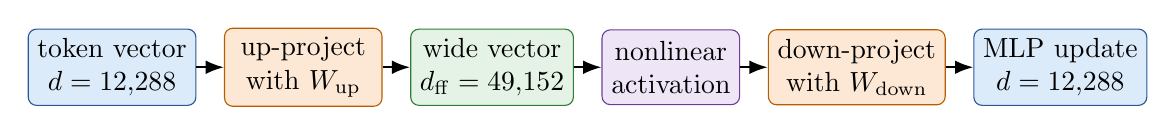
\begin{tikzpicture}[
      stage/.style={draw, rounded corners=3pt, minimum height=0.95cm,
        align=center},
      >=Latex
    ]
      \node[stage, minimum width=1.55cm, fill=tokenblue,
        draw=tokenblueborder] (input)
        {token vector\\\(d=12{,}288\)};
      \node[stage, minimum width=2.0cm, fill=tokenorange,
        draw=tokenorangeborder, right=0.35cm of input] (up)
        {up-project\\with \(W_{\mathrm{up}}\)};
      \node[stage, minimum width=1.7cm, fill=tokengreen,
        draw=tokengreenborder, right=0.35cm of up] (wide)
        {wide vector\\\(d_{\mathrm{ff}}=49{,}152\)};
      \node[stage, minimum width=1.25cm, fill=tensorpurple,
        draw=tensorpurpleborder, right=0.35cm of wide] (activation)
        {nonlinear\\activation};
      \node[stage, minimum width=2.0cm, fill=tokenorange,
        draw=tokenorangeborder, right=0.35cm of activation] (down)
        {down-project\\with \(W_{\mathrm{down}}\)};
      \node[stage, minimum width=1.55cm, fill=tokenblue,
        draw=tokenblueborder, right=0.35cm of down] (output)
        {MLP update\\\(d=12{,}288\)};
      \draw[->, thick] (input) -- (up);
      \draw[->, thick] (up) -- (wide);
      \draw[->, thick] (wide) -- (activation);
      \draw[->, thick] (activation) -- (down);
      \draw[->, thick] (down) -- (output);
    \end{tikzpicture}
  \end{center}

  \vspace{-0.5em}
  \begin{center}
    \scriptsize
    \renewcommand{\arraystretch}{1.3}
    \begin{tabular}{@{}lccc@{}}
      \toprule
      Matrix & Shape in one layer & Parameters per layer & Across 96 layers \\
      \midrule
      \(W_{\mathrm{up}}\) & \(12{,}288\times49{,}152\)
        & \(603{,}979{,}776\) & \(57{,}982{,}058{,}496\) \\
      \(W_{\mathrm{down}}\) & \(49{,}152\times12{,}288\)
        & \(603{,}979{,}776\) & \(57{,}982{,}058{,}496\) \\
      \bottomrule
    \end{tabular}
  \end{center}

  \vspace{-0.4em}
  \begin{alertblock}{Most GPT-3 parameters are in its MLPs}
    \centering
    Together: \(2\times57{,}982{,}058{,}496
      =115{,}964{,}116{,}992\) weights---about \(66\%\) of GPT-3.
  \end{alertblock}
\end{frame}

\begin{frame}{Model scale: GPT-3 175B (2020) vs. Gemma 4 31B (2026)}
  \small
  Both are Transformer models, but Gemma 4 reaches a much smaller parameter
  budget through a narrower, more modern architecture.

  \begin{center}
    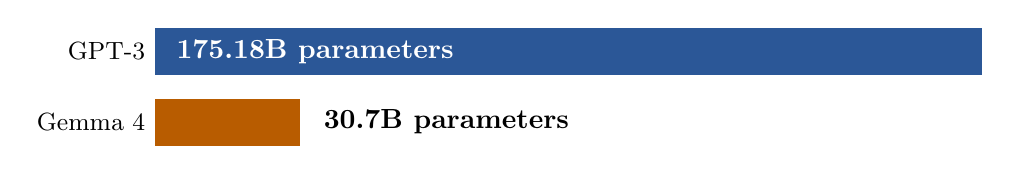
\begin{tikzpicture}[font=\small]
      \node[anchor=east] at (0,0.55) {GPT-3};
      \fill[tokenblueborder] (0,0.25) rectangle (10.5,0.85);
      \node[anchor=west, text=white, font=\bfseries]
        at (0.15,0.55) {175.18B parameters};

      \node[anchor=east] at (0,-0.35) {Gemma 4};
      \fill[tokenorangeborder] (0,-0.65) rectangle (1.84,-0.05);
      \node[anchor=west, font=\bfseries]
        at (2.02,-0.35) {30.7B parameters};
    \end{tikzpicture}
  \end{center}

  \vspace{-0.7em}
  \begin{center}
    \scriptsize
    \renewcommand{\arraystretch}{1.22}
    \begin{tabular}{@{}lrrrr@{}}
      \toprule
      Parameter family & GPT-3 175B & Share &
        \href{https://chatgpt.com/share/6a56a6e4-0c14-83ed-849e-93f362e5f1c3}{Gemma 4 estimate} & Share \\
      \midrule
      Embedding and output & \(1.24\)B & \(0.7\%\) & \(\approx1.41\)B & \(\approx4.6\%\) \\
      Attention: \(Q,K,V,O\) & \(57.98\)B & \(33.1\%\) & \(\approx6.10\)B & \(\approx19.8\%\) \\
      MLP: up and down projections & \(115.96\)B & \(66.2\%\) & \(\approx13.88\)B & \(\approx45.2\%\) \\
      Vision encoder and other weights & \(\approx0\)B & \(\approx0\%\) & \(\approx9.35\)B & \(\approx30.4\%\) \\
      \midrule
      \textbf{Total} & \textbf{175.18B} & \textbf{100\%} &
        \href{https://ai.google.dev/gemma/docs/core/model_card_4}{\textbf{30.7B}} & \textbf{\(\approx100\%\)} \\
      \bottomrule
    \end{tabular}
  \end{center}

  \vspace{-0.6em}
  \begin{alertblock}{About \(5.7\times\) fewer parameters}
    \footnotesize
    Gemma 4 uses 60 layers, a smaller embedding dimension, grouped-query and
    hybrid local/global attention, plus a vision encoder. Size alone is not a
    measure of capability; architecture, data, and training matter enormously.
  \end{alertblock}

\end{frame}


\section{Try it yourself}

\begin{frame}{Try it yourself: the \texttt{my-llm} notebook}
  The companion notebook turns the ideas from this presentation into a small,
  working Shakespeare language model.

  \vspace{0.6em}
  \begin{columns}[T]
    \begin{column}{0.48\textwidth}
      \begin{block}{What you will explore}
        \begin{itemize}
          \item character-level and BPE tokenization;
          \item training and validation batches;
          \item a small Transformer model;
          \item Shakespeare-like text generation.
        \end{itemize}
      \end{block}
    \end{column}
    \begin{column}{0.48\textwidth}
      \begin{block}{Get started}
        \begin{columns}[c,onlytextwidth]
          \begin{column}{0.62\linewidth}
            \footnotesize
            From the repository root, run:

            \smallskip
            \texttt{./setup.sh} (Linux/macOS), or

            \smallskip
            \texttt{.}\textbackslash\texttt{setup.ps1} (Windows PowerShell).

            \smallskip
            Then open \texttt{my-llm.ipynb}, select the project's
            \texttt{.venv} kernel, and run the cells from top to bottom.
          \end{column}
          \begin{column}{0.34\linewidth}
            \centering
            \begin{tikzpicture}
              \clip (0,0) rectangle (\linewidth,\linewidth);
              \node[anchor=north west,inner sep=0] at (0,\linewidth) {%
                \includesvg[width=20\linewidth]{assets/svg/qrcode}%
              };
            \end{tikzpicture}
          \end{column}
        \end{columns}
      \end{block}
    \end{column}
  \end{columns}

  \vfill
  \centering
  \small Start with the character tokenizer, then switch to BPE and compare
  the generated results.
\end{frame}

\begin{frame}{Dive deeper with 3Blue1Brown}
  \small
  Start with the short LLM primer between Chapters 4 and 5, then continue with
  Chapters 5 and 6 of 3Blue1Brown's \emph{Neural Networks} lecture series.

  \vspace{0.5em}
  \begin{columns}[T]
    \begin{column}{0.31\textwidth}
      \begin{block}{Start here}
        \centering
        \textbf{Large Language Models explained briefly}

        \smallskip
        \footnotesize
        A concise bridge from next-token prediction and training to
        Transformer architecture.
      \end{block}
    \end{column}
    \begin{column}{0.31\textwidth}
      \begin{block}{Chapter 5}
        \centering
        \textbf{Transformers and LLMs}

        \smallskip
        \footnotesize
        Tokens, embeddings, unembedding, softmax, and the overall architecture.
      \end{block}
    \end{column}
    \begin{column}{0.31\textwidth}
      \begin{block}{Chapter 6}
        \centering
        \textbf{Attention, step by step}

        \smallskip
        \footnotesize
        A visual walkthrough of queries, keys, values, and attention weights.
      \end{block}
    \end{column}
  \end{columns}

  \vfill
  \begin{center}
    \href{https://www.youtube.com/watch?v=LPZh9BOjkQs}{%
      \beamergotobutton{Watch Large Language Models explained briefly}}
    \hspace{0.7em}
    \href{https://www.youtube.com/playlist?list=PLZHQObOWTQDNU6R1_67000Dx_ZCJB-3pi}{%
      \beamergotobutton{Open the full playlist}}

    \medskip
    \scriptsize
    Both buttons are clickable in the PDF\@.
  \end{center}
\end{frame}

\begin{frame}[plain]
  \centering
  \Huge Questions?
\end{frame}

\end{document}
